\documentclass{article}
\usepackage{natbib}
\usepackage{hyperref}
\usepackage{times}
\usepackage[section]{placeins}
\usepackage{gensymb} % How can I write a \textdegree~ (degree) symbol in LaTeX?
%\graphicspath{ {/Videography_figures}}

\newcommand{\BibTeX}{{\sc Bib}\TeX}

\title{Santa Ana sucker Habitat Evaluation}
\author{C. Flynn, E. Harris-Tyrrell, L. Ho-Israel, O. Howie, S. Janssen, \\N. Larson, F. Lyles, W. Nore\~na, V. Sanchez-Jimenez, A. Vacas, D. Wagner,\\ Ed. Marc Los Huertos}

\usepackage{Sweave}
\begin{document}
\Sconcordance{concordance:Report_DRAFT.tex:Report_DRAFT.Rnw:%
1 11 1 1 0 228 1 1 5 5 1 1 5 6 1 1 4 7 1 1 4 13 1 1 5 10 1 1 4 3 1 1 4 %
116 1}


\maketitle

\newpage
\tableofcontents
\newpage

\section{Introduction}

\subsection{Scope of Problem}

The Santa Ana sucker (\emph{Catostomus santaanae}) is a relatively small fish extant in a few streams of Southern California. The species has been listed as threatened by the U.S. Fish and Wildlife Service, and has undergone a 70\% habitat loss \citep{obrien2011status, usfishandwildlifeservice14}. In addition to habitat loss, hydrodomodifications including the construction of flood control dams, stream channelization, groundwater extraction, and discharge of treated water, have profound effects on the river's hydrology and ecology. For example, water temperatures in portions of the Santa Ana river can range from 10 to 26\textdegree~C, however temperatures are noticeably elevated nearby areas of discharge due to the incorporated urban effluent \citep{greenfield70}. Additionally, wastewater discharge has been known to affect levels of dissolved oxygen in the water, potentially making it so that not enough oxygen is available for respiratory processes. Inadequate treatment techniques by the nearby treatment facility could affect sucker abundance, however optimal dissolved oxygen and biochemical oxygen demand levels have not been determined for the sucker \citep{baskerville2012recovery}. 

More recently, the abundance of the red alga \emph{Cosmopogen aeruginosus}, has increased significantly in the Santa Ana River. This may also be contributing to the sucker's decline, but the environmental variables that control the \emph{Cosmopogen aeruginosus}'s distribution in the Santa Ana River are currently not well understood. The direct effect this invasive algae has on \emph{C. santaanae} is also poorly constrained. 

In general, the environmental variables that influence \emph{C. santaanae} populations are poorly understood. Better understanding of water temperature, discharge rates, biochemicial oxygen demand (BOD), and \emph{Cosmopogen aeruginosus} distribution could aid in conservation efforts of this federally threantened fish. 

\subsection{Problem Statement}

This project began with the broad driving question, "How can the Santa Ana sucker be saved?" To that end, we have tried to constrain what environmental variables affect \emph{C. santaanae} distributions to water temperatures, BOD, (\emph{Cosmopogen aeruginosus} abundance, etc. 

\subsection{Background}

The geographic range of the Santa Ana sucker has declined from its historic distribution in the Los Angeles Basin \citep{brown2005aquatic, saiki2007life}. And within the Santa Ana River, the sucker habitat habitat is contrained some short reaches that are fed by treated discharges for most of the year --- in this context the river reach is highly modified in terms of it's hydrology, geomorphology,  water quality, and habitat characteristics--- becoming a disconnected stream \citep{poole2002fluvial}. 

\subsubsection{Stream Hydrology and Geomorphology}

Stream bed substract plays in important role in providing habitat for benthic dwelling fish, like the Santa Ana sucker. \citet{baskerville2012recovery} state that constant water flows are important to the availability of coarse substrate which the sucker needs to spawn offspring and hide from predators. According to \citet{evans2005long}, temporary reduction of flow, such as occurs when the treatment plant which now largely supplies the river halts releases of discharge water, can significantly reduce the habitat available for suckers. Just last month, the Center for Biological Diversity reported that "by halting water releases critical to maintaining surface flows of the Santa Ana River, the Rapid Infiltration and Extraction (RIX) treatment plant is stranding and killing threatened fish" \citep{evans2005draft}. 

Understanding the role of stream substrate can be important in restoring various fish populations. For example, restoration projects seemed to be failing to prevent the Chinook population from falling in the Merced River \citep{albertson13}. For example, the installation of gravel augmentation in a reconfigured channel seemed to have little impact on the salmon, suggesting that other factors were catalyzing the fall of the species. By comparing the restored portion with other portions of the Merced river, food web characteristics and flow discharge seemed to produce the same results on the various life stages of the salmon. However, higher temperatures, less woody debris, and minimal riparian cover seemed to limit populations in the restored portions. Restoration efforts are then presented with an added challenge of ensuring that every aspect of the ecosystem is beneficial to the species, which demands more work toward temperature regulation and attempts to restore the river bank. To see how the Santa Ana sucker would react to similar conservation efforts would be interesting in discussions in attempting to determine solutions.

\subsection{Water Quality}

Water temperature can influence sucker habitat value. For example, Moyle postulates that the sucker prefers environments with cool water \citep{moyle2002inland}. Again, the temperature of the Santa Ana River has been rising to levels greater than the sucker could stand \citep{REF}. Other types of fish have been known to regulate their body temperatures by moving to different areas in their habitat throughout the day \citep{matthews1994cool}. Temperature can play a signficant role fish behavior. For example, \citet{sadler1980effect} found discharge downstream of a impoundment altered fish populiaton densities as a result of temperature. Human activities can increase water temperature. Water-based organisms are sensitive to temperature change, especially young fish due to limited mobility. The effect of temperature on fish varies greatly depending on other conditions of the lake or river environment of the fish in question \citep{loshuertos16}. Heat, temperature, thermal energy, and heat capacity all slightly change how heat is measured in an ecosystem. Water in general has a high heat capacity, which indicates its high specific heat. Thus, aquatic systems therefore often retain their heat and are less susceptible to changes in temperature than non-aquatic systems. Inflows/mixing can have an effect on water temperature but it is often hard to detect due to thermal stratification mixing, seasonal change in temperature profile depth, and small volume inflow in terms of fraction of the lake volume. Temperature impacts many other features of water quality, which will be important to keep in mind going forward with the project. \citet{coulter2015fluctuating} explain how young Flathead Minnows exposed to warmer temperatures underwent a nondirectional sex reversal . This paper shows us how temperature can greatly affect fish and stress them out. 

In addition, evidence suggests that the RIX discharge waters affect the growth and development of the of mosquito fish (xxx) and the Santa Ana sucker \citep{jenkins2009effects}. For example, fish have been known to be at risk of suffocation when exposed to dissolved oxygen (DO) levels below 2 mg/L for only short periods of time \citep{REF}. A 2012 U.S. Fish and Wildlife Service report on the recovery of the endangered fish noted that specific tolerances to dissolved oxygen have not been determined for  Santa Ana sucker \citep{evans2005draft}.

\subsubsection{Community Ecology}

For the Santa Ana River sucker habitat, a central threat is the invasive \emph{Cosmopogen aeruginosus} that has been spreading with alacrity in areas where the fish are known to be, including the reach below the Rapid Infiltration and Extraction (RIX) Treatment plan (Palenscar).There are concerns that the algae may be one of the contributing factors to the sucker's decline. For example, one of the important features of the Santa Ana River for the sucker is the presence of coarse substrate i.e., gravel and cobble as opposed to silt and sand \citep{thompson2010influence}. The sucker has adapted to feeding on the diatoms that tend to grow on the former. 

Algae biomass can depend on a range of variables, both biotic and abiotic \citep{winkelmann2014top}. In general, diatom growth dominance has been associated with high quality sucker habitat \citep{REF}. However, an introduced red alga, \emph{Cosmopogen aeruginosus}, may be displacing diatom food sources. 

Although the introduction of the \emph{Cosmopogen aeruginosus} are not unique to the Santa Ana River \citep{vzakova2013new}, few locations have documented the ecological impact of its presence. Some of the diatoms on which the sucker feeds may be able to grow on the algae (are epiphytic), thus have limited impact on the sucker. Alternatively, \emph{Cosmopogen aeruginosus} may displace diatoms and detritus, on which the sucker relies \citep{thompson2010influence}. In addition, if the sucker is ingesting the algae, this may constitute a factor to the sucker's decline. Of course, ingesting the algae is not a necessity to the fish being negatively impacted; the algae may also disrupt the fish's well-being in unknown ways. 

\subsection{Objectives}
This experiment explores sevreal aspects of \emph{C. santaanae} habitat and distribution. Using measurments of river water temperature, overhead tree canopy cover, and sediment type we explore the environmental variables of the river and their relationship with the distribution of \emph{Cosmopogen aeruginosus}. Our second goal of this study is to discover whether or not the Santa Ana suckers are coping with this dramatic increase in temperature by moving to cooler sections of the stream throughout the day, by recording video footage of \emph{C. santaanae} movement. 

Our goal with this experiment was to find out whether or not temperature was affecting the population and/or livelihood of the Santa Ana sucker in the Santa Ana River.

Our goal is to obtain footage clearly showing the density of Santa Ana suckers in the different locations at different points in the day.  We hope to get accurate enough footage to count the number of fish in each video, then run an ANOVA test on each location to see if the quantity of fish significantly varies at different times of the day.  If they do, we will be able to conclude that the suckers move throughout the day to find their preferred temperature.

Does the Santa Ana sucker shift its distribution in the Santa Ana River based on natural temperature changes that occur throughout the day? We believe that if we monitor the relative distribution of the Santa Ana suckers throughout the day we will see a difference in sucker abundance between an upstream and downstream location in response to changing temperature throughout a 24-hour period.

Finally, this report aims to determine whether Biochemical Oxygen Demand (BOD) and water flow velocity are relevant to future research regarding the endangered Santa Ana sucker \emph{C. santaanae}. We collected water quality data from the Santa Ana River to answer the following questions: \emph{Do BOD levels vary in different sections of the river}; \emph{Do differing BOD levels correlate with the abundance of individuals?}; and \emph{Do the water flow rates in different sections of the river correlate with sucker populations?} Because the section of the river we evaluated regularly receives discharge water from a nearby water treatment facility, we believe that BOD levels will be relatively low, around 10 mg/L, decreasing further from the discharge point. Where the BOD levels are lower, we expect higher fish count. We also hypothesize that larger populations of the sucker will concentrate near high-flow sections. Through this experiment, we aim to inform Santa Ana sucker conservation efforts and hope to inform action by the nearby water treatment facility. 

The presence of the non-native \emph{Cosmopogen aeruginosus} in the Santa Ana River and the possible relationship it holds with Santa Ana sucker's decline. In the last five years, the non-native tropical \emph{Cosmopogen aeruginosus} Cosmopogen Aeruginosus has been found in large quantities in the Santa Ana River. Using measurements of river water temperature, overhead tree canopy cover, and sediment type, we explore the connection these aspects of the river and their relationship with the \emph{Cosmopogen aeruginosus}.

\begin{quote}
Our null hypotheses are H0: Water flow velocity and/or BOD levels do not significantly correlate with prevalence of the Santa Ana sucker.
\end{quote}
\begin{quote}
Our alternative hypotheses are H1: Water flow velocity and/or BOD levels significantly correlate with prevalence of the Santa Ana sucker.
\end{quote}
If we can reject one or both of our null hypotheses, we can conclude that the study of Biological Oxygen Demand (BOD) and water flow velocity are relevant to future conservation research for the endangered Santa Ana sucker \emph{C. santaanae}.


\section{Methods}

\subsection{Materials and Equipment}
\begin{itemize}
\item 2 Waterproof GoPro "Hero 4 Silver" cameras with mounts, and 4 64GB microSD SanDisk memory cards
\item 4 Waterproof Re-Fuel 6-Hour ActionPack Battery (DigiPower)
\item 2 Grey Cinder block backs, ~8in x 8in
\item Original Sticks to Everything Gorilla Glue
\item 4 HOBO Tidbit Water Temperature Data Logger,
\item 1 Optic USB U-4 Base Station with coupler and HOBOware software,
\item 4 Green Garden stakes to hold loggers in stream channel
\item Red flags, Yellow marking tape,
\item GPS Spherical Canopy Densiometer
\item 30cm x 30cm PCV Quadrat
\item Meter tape
\item Write-in-the-Rain field books
\item snorkleing goggles 
\end{itemize}

\subsection{Site Description}

We evaluated the Santa Ana River near Colton, California (Figure \ref{SAR_Image}) along Aqua Mansa Road between S Riverside Ave. and S. Rancho Ave in Rialto, California.  We collected data from four reaches, one on the Rialto Channel and the other three in the Santa Ana river (Figure \ref{SAR_Image}). 

The specific sites for our project consisted of one upstream location (Site 1) and one downstream location (Site 4), located roughly one kilometer apart (Table \ref{tab:sitedescription}). Site 2 was located just below the Rialto concrete channel and Site 4 was a plunge pool. The upstream location had large debris like rocks and branches. The downstream location was smooth and flat, with a bed of pebbles and smaller coarse sediments. 

\begin{table}
\caption{Description of sampling locations.}
\begin{tabular}{llll}\hline
Location & Latitude             & Longitude   & Description \\ \hline\hline
Site 1  &  TBD  & TBD  & Rialto Channel \\
Site 2  & 34\textdegree 2'29"N          & 117\textdegree 21'15"W   & Above RIX Influx \\
Site 3  & 34\textdegree 2'21"N          & 117\textdegree 21'20"W   & Below RIX Influx\\
Site 4  & 34\textdegree 2'5"N           & 117\textdegree 21"17"W   & Pool, approximately 40-50 cm in depth\\ \hline
\end{tabular}
\label{tab:sitedescription}
\end{table}


The river was surrounded by a derelict lot filled with trash. It was very industrial, with many trucks idling by the roadside and industrial shipping buildings. Rip-rap to protect the channel levy. The area we walked through to approach the river was very sandy, with tire tracks. The river itself had some trash in it and was smaller than expected in contrast to rivers in other areas of the country, like the Pacific Northwest. 


\begin{figure}[!ht]
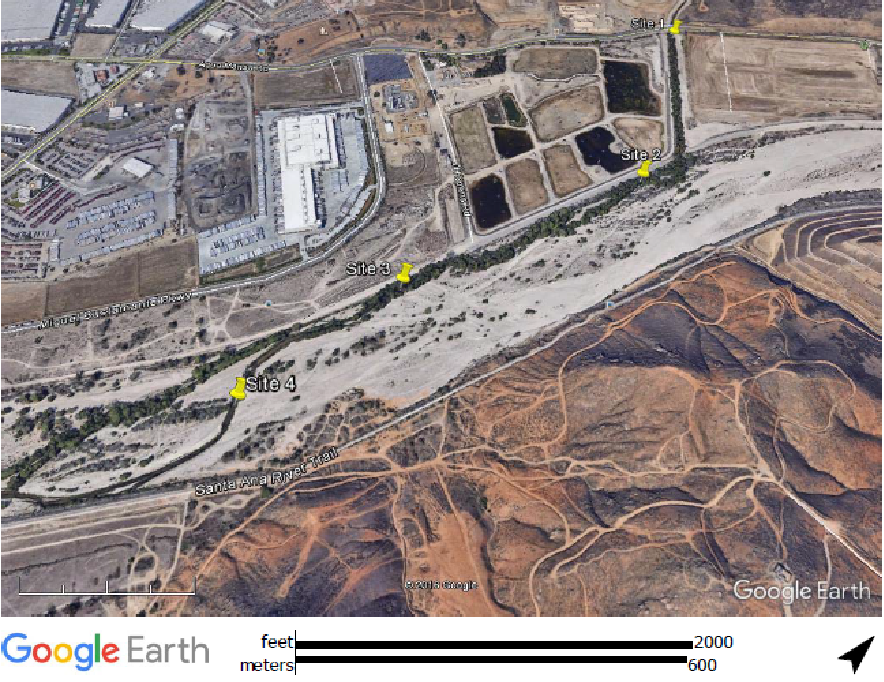
\includegraphics[width=1.00\textwidth]{Figures/SiteMap}
\caption{Sampling location maps}
\label{SAR_Image}
\end{figure}

\subsection{Habitat Evaluation}

The collection of data on the algae abundance, sediment type, and vegetation canopy cover of the Santa Ana River was done along the section of the river described in the site description section on September 20th, 2016, from 1pm to 3:30pm. We evaluated 9 parameters from Sites 2-4, for a total of 27 measurements. At each site, beginning at Site 4, the following procedures were followed: 

\begin{enumerate}
\item A spot was chosen along the right bank. Each of the parameters were then measured.
\item For estimating algae abundance, we placed the 30  x 30 cm quadrat above the river bed and estimated the \% that was covered by algae to the nearest 10 \%.

\item The sediment type of the site was characterized as either fine or coarse based on the grain size of the 30x30cm section of stream bed covered by the quadrat as either fine or coarse. Coarse substrate was classified as anything larger than pebbles or sand, that is, larger than 6.5cm. If more than half of the area covered by the quadrat was coarse substrate, or fine substrate, the area was characterized as such respectively.

\item Canopy cover was measured from the same position as the algae by holding spherical canopy densiometer above water at elbow's length. Based on how many of the 15 intersections on the densiometer reflected overhead canopy, cover was then quantified on a 0-15 scale, 0 being the no canopy cover and 15 being full cover.

\item To measure temperature, we submerged the analog thermometer underwater and recorded the temperature in degrees Celsius.

\item Qualitative aspects of the river, such as presence of a pool or of logs, were also noted at each measurement spot.

\item Each measurement was then also taken at the middle of the river and the left bank of the cross-section. 

\item Steps above were repeated at two cross-sections between 0 and 10 meters downstream both chosen using a random number generator for a total of 3 cross-sections along a possible total length of 20 meters, and 3 measurements at each cross-section, for a total of 9 measurements per site. 
\end{enumerate}

At each of the corresponding water sample collection sites, water velocity was also measured using a SonTek FlowTracker Handheld Advanced probe, which emits sonar waves at a certain depth in the water column, and based on the feedback (20 pings) gives a velocity reading. Ideally, multiple readings would be taken at each site, after the probe is placed on a flat section of the riverbed where water appears to be flowing net in the same direction. 

\subsection{Videography}

We acquired all the necessary equipment for an underwater filming project, keeping in mind the length of time we wanted to keep our cameras underwater. We chose the GoPro Hero 4 Silver because of its battery life and recording time. We also considered safety and theft prevention for the cameras, and for this reason decided to mount the cameras in cube-shaped cinderblock structures with one open side that we constructed ourselves. In the lab, we set up all the equipment, built the cinderblock structures, and prepared everything for the field. Once in the field, we selected appropriate data sites (sites 2 and 4), set up our cameras, and set them to record at morning and afternoon times throughout the day. After the data collection period, we collected the equipment from the river and did a fish count analysis of all the footage back in the lab. Initially, we tried counting the fish by placing an arbitrary line in the footage and only counting in that area. We counted during an interval of ten seconds As can be seen in Figure \ref{fig:wherefish}, fish were very hard to see in the footage. We later did a recount and counted all the visible fish in the video frame every minute for one hour of footage each in the morning and afternoon. More detailed information on these processes can be found in the appendix.
\begin{figure}
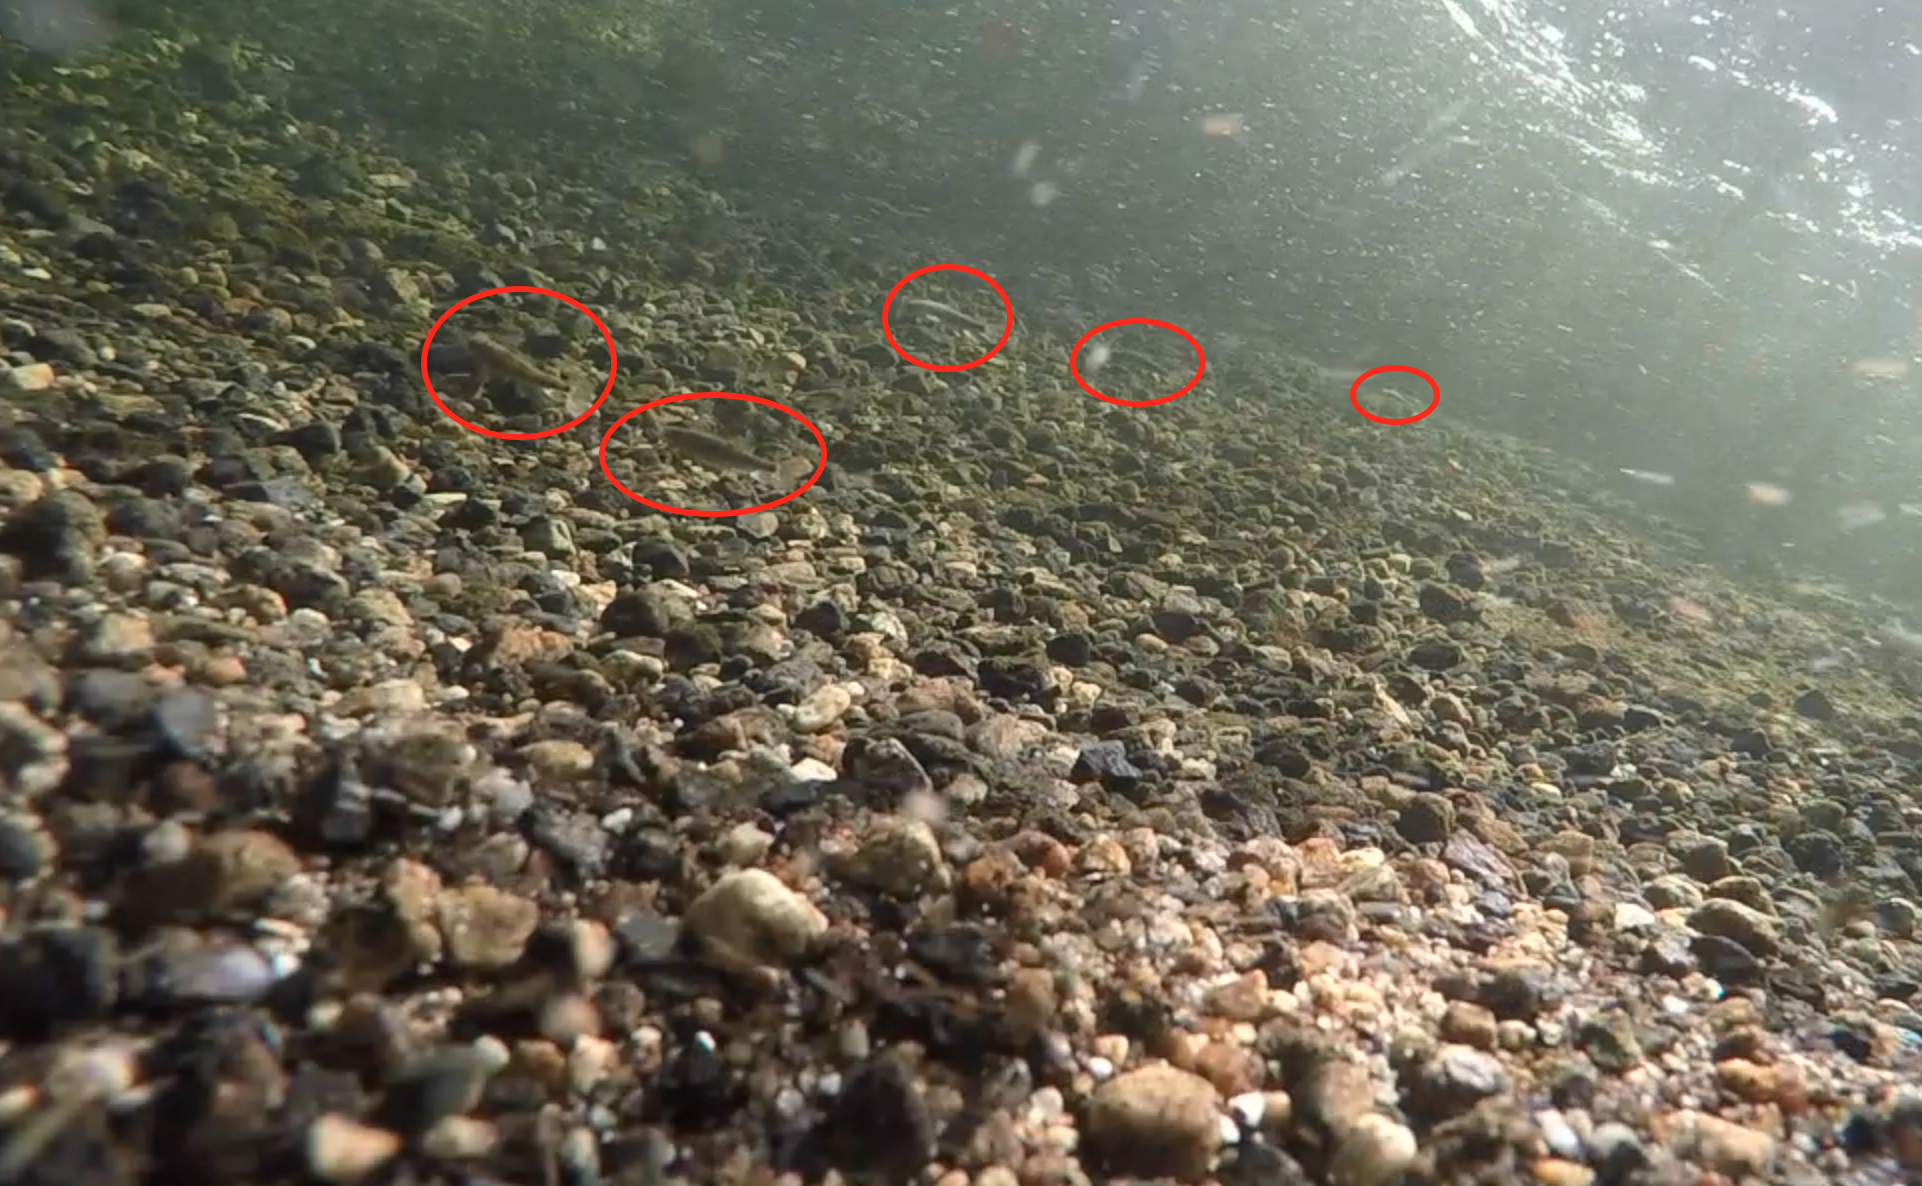
\includegraphics[scale=.4]{Videography_figures/wherefish}
\caption{The Santa Ana suckers were difficult to see in the underwater footage. Here, a few fish have been circled in the frame to showcase this. Because the fish were only clearly visbile when they were moving, it was necessary to count during a 10 second interval of footage.}
\label{fig:wherefish}
\end{figure}

\subsection{Temperature Loggers}

Temperature collection occurred from September 25th til October 1st for Site 2, and September 25th til October 4th for Sites 1, 3, and 4, every 15 minutes. We programmed the loggers via our base station and the HOBOware software to collect water temperature data every 15 minutes. After collecting the field data, we calibrated the loggers by putting them in an ice bath for several minutes to ensure that the temperature settled around zero and each logger was measuring to the same temperature with the same accuracy.

\subsection{BOD Methods}

Approximately 1L of source river water was collected at each of two sites, one upstream location (Site 2) closer to the wastewater discharge facility, and one downstream location (Site 4). Ideally, these would be transported to the laboratory for analysis within four hours. BOD was carried out using the following methods...\textbf{[need to add method to report.bib]}

\subsection{Statistical Methods}

Using the R programming environment \citep{CRAN}, we use linear regression and ANOVA to analyze stream habitat variables. We also tested habitat value with fish count data comparing morning to afternoon counts. However, we acknowledge the fish count data are spatially and temporally autocorrelated, thus, our conclusions we make are serverely constrained based on the sampling methods.

\section{Results}

